\documentclass[conference]{IEEEtran}
\IEEEoverridecommandlockouts

\usepackage{cite}
\usepackage{amsmath,amssymb,amsfonts}
\usepackage{graphicx}
\usepackage{textcomp}
\usepackage{xcolor}
\usepackage{booktabs}
\usepackage{multirow}
\usepackage{tikz}
\usetikzlibrary{arrows.meta,positioning}
\usepackage[hidelinks]{hyperref}

% ------------------------------------------------------------------
%  AUTHOR DETAILS -- edit these five lines only
% ------------------------------------------------------------------
\newcommand{\authorname}{Your Name}
\newcommand{\authordept}{Department of Computer Science and Engineering}
\newcommand{\authorinst}{Your College / University}
\newcommand{\authorcity}{City, Country}
\newcommand{\authoremail}{your.email@example.com}
% ------------------------------------------------------------------

\newcommand{\nSeeds}{5}
\newcommand{\trainWindows}{10080}
\newcommand{\testWindows}{4320}
\newcommand{\cgP}{0.95}
\newcommand{\cgR}{0.96}
\newcommand{\cgFone}{0.95}
\newcommand{\cgAUC}{0.98}
\newcommand{\cgDet}{100}
\newcommand{\cgDetStealthy}{100}
\newcommand{\cgTTDnoisy}{1.4}
\newcommand{\cgTTDstealthy}{16}
\newcommand{\cgTTDcontainer}{3.3}
\newcommand{\cgFA}{0.13}
\newcommand{\cgHN}{0.0}
\newcommand{\nomwFone}{0.78}
\newcommand{\nomwTTDstealthy}{134}
\newcommand{\nomwDetStealthy}{90}
\newcommand{\ocFone}{0.91}
\newcommand{\ocFA}{2.47}
\newcommand{\ocHN}{96}
\newcommand{\ocDet}{100}
\newcommand{\stDet}{61}
\newcommand{\stFone}{0.46}
\newcommand{\stFA}{1.67}
\newcommand{\sigDet}{63}
\newcommand{\sigFone}{0.70}
\newcommand{\ifFone}{0.44}
\newcommand{\ifFA}{2.20}
\newcommand{\ifHN}{97}
\newcommand{\respContain}{100}
\newcommand{\respTTC}{12.5}
\newcommand{\respWrongKill}{0.00}
\newcommand{\respWrongIso}{0.00}
\newcommand{\shareMinerMin}{0.86}
\newcommand{\shareSurge}{0.41}
\newcommand{\shareCI}{0.64}
\newcommand{\exStealthyMinute}{16}
\newcommand{\exStealthySummary}{Looks like cryptojacking because the server is using 30 percentage points more CPU than its current traffic and process activity can explain (normally under 5); a single process is using 30\% of total CPU (normal top process: $\sim$9\%); one process accounts for 70\% of all CPU use (normally $\sim$40\%).}
\newcommand{\liveNoisyKill}{0.8}
\newcommand{\liveStealthyKill}{92}


\begin{document}

\title{CryptoGuard: Explainable, Self-Responding Detection of Cryptojacking on Cloud Servers}

\author{\IEEEauthorblockN{\authorname}
\IEEEauthorblockA{\authordept\\
\authorinst\\
\authorcity\\
\authoremail}}

\maketitle

\begin{abstract}
Cryptojacking---secretly running cryptocurrency miners on someone else's cloud servers---steals no data and triggers few security alarms, so it is often discovered only when an unexplained cloud bill arrives. This paper presents CryptoGuard, a host-level system that learns the normal behaviour of a cloud server from its CPU, process and network telemetry, detects mining-like deviations in real time, explains every alert in plain language, and automatically contains the threat. CryptoGuard combines four ideas: (i) a learned \emph{CPU-excess} feature that measures how much CPU the server is using beyond what its current workload explains; (ii) an Isolation Forest for abrupt anomalies together with a CUSUM accumulator for throttled, low-and-slow miners; (iii) an \emph{explanation-guided gate} that uses TreeSHAP attributions to separate compute-driven (mining-like) anomalies from benign workload changes such as traffic surges and build jobs; and (iv) a graduated responder that alerts, terminates the attributed process tree, or quarantines the server according to a fused confidence score. On a simulated cloud-server workload with three attack families and two kinds of legitimate heavy load, evaluated over \nSeeds{} random seeds, CryptoGuard detected \cgDet\% of attacks with an F1-score of \cgFone{}, \cgFA{} false alerts per day and no alerts on the benign heavy workloads, whereas a static CPU alarm detected \stDet\% of attacks and a One-Class SVM alerted on \ocHN\% of benign heavy-load windows. In a live test with a harmless miner simulator, CryptoGuard automatically terminated a noisy miner \liveNoisyKill{}\,s after it started and a throttled, signature-free miner after \liveStealthyKill{}\,s.
\end{abstract}

\begin{IEEEkeywords}
cryptojacking, cloud security, anomaly detection, explainable AI, SHAP, isolation forest, CUSUM, automated incident response
\end{IEEEkeywords}

% ==================================================================
\section{Introduction}
% ==================================================================
Organisations increasingly run their applications on rented cloud servers that are billed by the amount of compute they consume. That billing model has created a profitable target for attackers: instead of stealing data, an intruder who obtains access to a cloud account or a misconfigured instance installs a cryptocurrency miner and lets the victim pay for the electricity and hardware. Google's Cybersecurity Action Team reported that 86\% of 50 recently compromised Google Cloud instances were used for cryptocurrency mining, in many cases within seconds of the compromise~\cite{google2021threat}. Sysdig's threat research team estimated that victims are billed about \$53 in cloud resources for every \$1 of cryptocurrency the attacker earns~\cite{sysdig2022}. MITRE ATT\&CK catalogues the behaviour as \emph{Resource Hijacking}~\cite{mitre_t1496}.

Cryptojacking is hard to catch with conventional tools because nothing that those tools look for actually happens. No files are exfiltrated, no ransom note appears, and no password is brute-forced after the initial intrusion; the only symptom is that the server quietly works harder than it should. Signature-based defences that match miner binaries or mining-pool addresses are easily evaded by renaming the binary and tunnelling the Stratum protocol over TLS on port 443~\cite{tekiner2021sok,pastor2020}. Static cloud alarms such as ``CPU above 90\% for five minutes'' miss miners that throttle themselves, and they fire on every legitimate busy period.

This work builds a system that behaves more like a doctor who knows a patient's normal heartbeat. CryptoGuard first learns what normal behaviour looks like for a particular server, then watches it continuously. When it sees a deviation, it does not simply log ``anomaly detected''; it states \emph{why} the behaviour looks like mining, for example ``the server is using 30 percentage points more CPU than its current traffic can explain and a single process is responsible for most of it''. When its confidence is high enough, it acts immediately by terminating the culprit process or isolating the server, while notifying a human to investigate.

The contributions of this paper are:
\begin{enumerate}
  \item A host-telemetry feature set for cryptojacking that includes a learned \emph{CPU-excess} signal: the CPU utilisation not explained by the server's current network and process workload.
  \item A two-time-scale detector that pairs an Isolation Forest~\cite{liu2008iforest} for abrupt anomalies with a CUSUM accumulator~\cite{page1954} for throttled miners whose individual windows look only mildly unusual.
  \item An \emph{explanation-guided gate} that uses exact TreeSHAP attributions~\cite{lundberg2017,lundberg2020trees} not only to explain alerts to an administrator, but also to decide whether an anomaly is mining-like. Anomalies explained by traffic or process churn are reported without triggering a response.
  \item A graduated, safety-railed automated responder (alert, kill, isolate) with evidence fusion from threat intelligence, process attribution, allow-lists, dry-run mode and an audit log.
  \item An open implementation with a reproducible evaluation harness, ablation study and live test.
\end{enumerate}

% ==================================================================
\section{Related Work}
% ==================================================================
\textbf{Cryptojacking.} Tekiner et al.~\cite{tekiner2021sok} systematise cryptojacking malware and its detection, and report that most proposed detectors rely on a small set of features and assume no evasion. Early academic work focused on in-browser mining: Eskandari et al.~\cite{eskandari2018} gave a first measurement of browser-based cryptojacking, and Konoth et al.~\cite{konoth2018minesweeper} proposed MineSweeper, which detects WebAssembly miners from their cryptographic primitives and cache behaviour. Cloud and container cryptojacking, where the miner is an ordinary native process, has received less academic attention despite being the dominant real-world payload on compromised cloud instances~\cite{google2021threat,sysdig2022}.

\textbf{Network-based detection.} Pastor et al.~\cite{pastor2020} detect encrypted mining connections from flow features with machine and deep learning. Network detectors are complementary to CryptoGuard: they need flow-level visibility and labelled mining traffic, while CryptoGuard needs only the host's own telemetry and no attack labels.

\textbf{Anomaly detection and explainability.} Unsupervised anomaly detection~\cite{chandola2009} is attractive for cryptojacking because labelled attacks on a specific server are rarely available. Isolation Forest~\cite{liu2008iforest} and One-Class SVM~\cite{scholkopf2001} are standard choices. Their alerts are, however, hard to act on without explanations. Model-agnostic methods such as LIME~\cite{ribeiro2016} and SHAP~\cite{lundberg2017} attribute a prediction to input features, and TreeSHAP~\cite{lundberg2020trees} computes exact Shapley values for tree ensembles in polynomial time. Most prior work uses explanations only for presentation; CryptoGuard additionally feeds the explanation back into the decision.

% ==================================================================
\section{Threat Model}
% ==================================================================
The defender operates Linux cloud servers (virtual machines or containers) and can run an agent on each. The attacker has gained code execution on a server, for example through weak credentials, a vulnerable service or an exposed container API, and runs a CPU miner. The attacker may (a) rename the miner binary, (b) reach the pool over TLS on port 443 or through a proxy, (c) throttle the miner to a fraction of the CPU, and (d) spawn the miner from a container with many short-lived helper processes. The attacker does not tamper with the agent itself; agent hardening is out of scope. The defender must avoid disrupting legitimate workloads, which include daily backups, weekly batch jobs, traffic surges and CI builds.

% ==================================================================
\section{System Design}
% ==================================================================
\begin{figure*}[t]
  \centering
  \resizebox{\textwidth}{!}{% CryptoGuard architecture (TikZ). Included from paper.tex as a two-column figure.
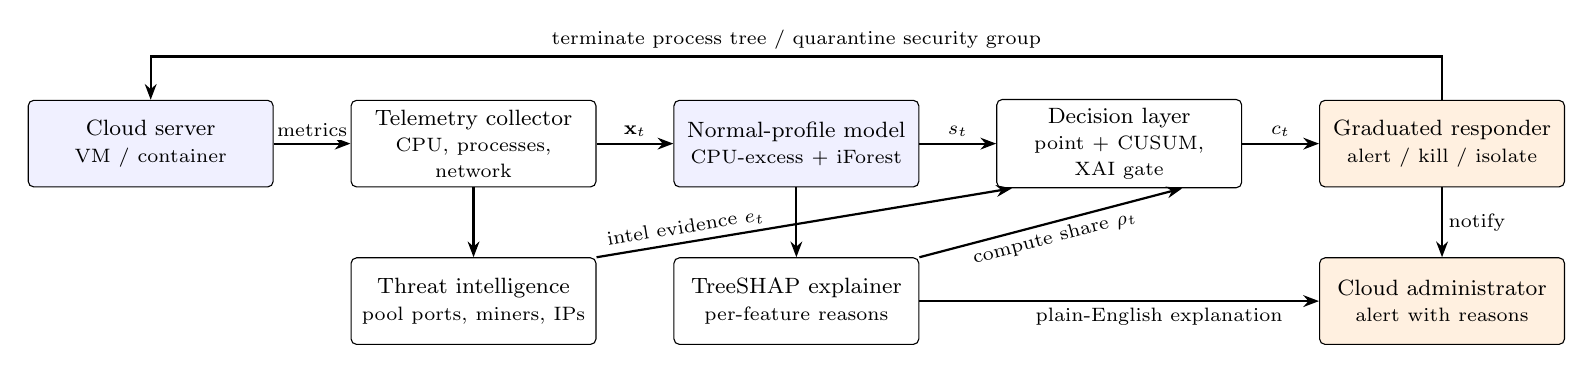
\begin{tikzpicture}[
  font=\footnotesize,
  box/.style={draw, rounded corners=2pt, align=center, minimum height=11mm, text width=29mm, execute at begin node={\hyphenpenalty=10000\exhyphenpenalty=10000},
              inner sep=3pt, fill=white},
  arr/.style={-{Stealth[length=2mm]}, thick},
  lab/.style={font=\scriptsize, fill=white, inner sep=1pt}]
  \node[box, fill=blue!6]  (host)  at (0,0)    {Cloud server\\\scriptsize VM / container};
  \node[box]               (col)   at (4.1,0)  {Telemetry collector\\\scriptsize CPU, processes, network};
  \node[box, fill=blue!6]  (model) at (8.2,0)  {Normal-profile model\\\scriptsize CPU-excess + iForest};
  \node[box]               (det)   at (12.3,0)  {Decision layer\\\scriptsize point + CUSUM, XAI gate};
  \node[box, fill=orange!12](resp) at (16.4,0) {Graduated responder\\\scriptsize alert / kill / isolate};
  \node[box]               (ti)    at (4.1,-2) {Threat intelligence\\\scriptsize pool ports, miners, IPs};
  \node[box]               (xai)   at (8.2,-2) {TreeSHAP explainer\\\scriptsize per-feature reasons};
  \node[box, fill=orange!12](admin) at (16.4,-2) {Cloud administrator\\\scriptsize alert with reasons};

  \draw[arr] (host) -- node[lab, above=1pt]{metrics} (col);
  \draw[arr] (col) -- node[lab, above=1pt]{$\mathbf{x}_t$} (model);
  \draw[arr] (model) -- node[lab, above=1pt]{$s_t$} (det);
  \draw[arr] (det) -- node[lab, above=1pt]{$c_t$} (resp);
  \draw[arr] (col) -- (ti);
  \draw[arr] (model) -- (xai);
  \draw[arr] (ti.north east) -- node[lab, pos=0.22, sloped, above=1pt]{intel evidence $e_t$} ([xshift=2mm]det.south west);
  \draw[arr] (xai.north east) -- node[lab, sloped, below=1pt]{compute share $\rho_t$} ([xshift=8mm]det.south);
  \draw[arr] (resp) -- node[lab, right=1pt]{notify} (admin);
  \draw[arr] (xai.east) -- node[lab, pos=0.6, below=1pt]{plain-English explanation} (admin.west);
  \draw[arr] (resp.north) -- ++(0,0.55) -| node[lab, pos=0.25, above=1pt]{terminate process tree / quarantine security group} (host.north);
\end{tikzpicture}
}
  \caption{CryptoGuard architecture. Each observation window flows from left to right; the explainer and the threat-intelligence module feed evidence into the decision layer, and the responder closes the loop on the server.}
  \label{fig:arch}
\end{figure*}

Fig.~\ref{fig:arch} shows the pipeline. Every window $t$ (10\,s in live mode, 1\,min in the simulation), the collector produces a feature vector $\mathbf{x}_t$; the model scores it; the decision layer combines the score with SHAP-based and threat-intelligence evidence into a confidence $c_t\in[0,1]$; and the responder acts on $c_t$.

\subsection{Telemetry and Features}
The collector uses \texttt{psutil} to sample CPU utilisation once per second within each window and to enumerate processes and established TCP connections. Table~\ref{tab:features} lists the features. Behavioural features are fed to the anomaly model. Threat-intelligence features are zero on almost every healthy window, so a model trained on normal data could not learn from them; they are fused with the model output instead (Section~\ref{sec:fusion}).

\begin{table}[t]
\caption{Features computed for every observation window}
\label{tab:features}
\centering
\footnotesize
\begin{tabular}{@{}lp{4.3cm}@{}}
\toprule
Feature & Meaning \\
\midrule
\multicolumn{2}{@{}l}{\emph{Behavioural (model input)}}\\
\texttt{cpu\_percent} & mean CPU utilisation in the window \\
\texttt{cpu\_std} & CPU variability; miners keep the curve flat \\
\texttt{cpu\_sustained} & share of the last 10 windows above 80\% CPU \\
\texttt{top\_proc\_cpu} & CPU of the most CPU-hungry process \\
\texttt{top\_proc\_share} & that process's share of all CPU in use \\
\texttt{mem\_percent} & memory utilisation \\
\texttt{num\_procs}, \texttt{new\_procs} & running and newly spawned processes \\
\texttt{net\_conns}, \texttt{unique\_ips} & established connections, distinct peers \\
\texttt{bytes\_out}, \texttt{bytes\_in} & network throughput (kbps) \\
\texttt{hour\_sin}, \texttt{hour\_cos} & time of day on the unit circle \\
\texttt{cpu\_excess} & learned: CPU not explained by workload, (\ref{eq:excess}) \\
\midrule
\multicolumn{2}{@{}l}{\emph{Threat intelligence (fused)}}\\
\texttt{pool\_port\_conns} & connections to Stratum ports (3333, 4444, 14444, \ldots) \\
\texttt{miner\_name\_hits} & name/cmdline matches (xmrig, minerd, stratum+tcp, \ldots) \\
\texttt{blocklist\_ip\_conns} & connections to known pool / proxy IPs \\
\bottomrule
\end{tabular}
\end{table}

\subsection{Normal-Profile Model}
\textbf{CPU excess.} On a healthy server, CPU is driven by work: requests, connections, transfers and processes. CryptoGuard fits a ridge regression $f_\theta$ from the workload vector $\mathbf{w}_t$ (connections, peers, bytes in/out, new and running processes, time of day) to CPU utilisation $u_t$ on normal data and defines
\begin{equation}
  e_t = \max\!\big(0,\; u_t - f_\theta(\mathbf{w}_t)\big).
  \label{eq:excess}
\end{equation}
The feature is one-sided on purpose: a miner only ever \emph{adds} CPU, while using less CPU than expected is harmless. A linear model is used because it extrapolates sensibly to traffic levels never seen during training; a tree model would cap its prediction at the training maximum and make every traffic surge look like excess CPU.

\textbf{Isolation Forest.} The behavioural features, including $e_t$, are robust-scaled and modelled by an Isolation Forest with 300 trees and sub-samples of 2048 windows. The anomaly score is the original Isolation Forest score $s_t = 2^{-\mathbb{E}[h(\mathbf{x}_t)]/c(\psi)}$, where $h$ is the path length, $c(\psi)$ its expected value for a sub-sample of size $\psi$, and higher means more anomalous~\cite{liu2008iforest,pedregosa2011}. The point-anomaly threshold $\tau$ is the 99.5th percentile of scores on a separate day of normal calibration data, and $m$ and $\sigma = Q_{0.95}-m$ are the median and upper spread of those scores.

\subsection{Two-Time-Scale Decision}
\textbf{Point anomalies.} A window is a point anomaly when $s_t>\tau$. To suppress isolated spikes, the behavioural evidence only counts once $k=3$ of the last $n=5$ windows are mining-like point anomalies. Its confidence is $b_t = \tfrac12 + \tfrac12\tanh\!\big((s_t-\tau)/\sigma\big)$, which equals 0.5 at the threshold.

\textbf{Drift anomalies.} A miner throttled to 20--35\% of the CPU produces windows whose scores lie only slightly above normal. CryptoGuard accumulates such evidence with a one-sided CUSUM~\cite{page1954} on the standardised score $z_t=(s_t-m)/\sigma$:
\begin{equation}
  S_t = \min\!\Big(h + 5\kappa,\; \max\!\big(0,\; S_{t-1} + g_t\,[\min(z_t, z_\tau) - \kappa]\big)\Big),
  \label{eq:cusum}
\end{equation}
where $\kappa=1$ is the allowance, so only windows above the 95th percentile of normal add evidence. The increment is clipped at $z_\tau=(\tau-m)/\sigma$ because strong anomalies are already handled by the point detector. The cap $h+5\kappa$ lets the alarm clear a few windows after an attack stops. The gate $g_t\in\{0,1\}$ removes evidence from windows that the XAI gate rejects or that fall inside a registered maintenance window. The decision interval $h$ is set to 1.2 times the largest value of $S_t$ reached on all normal training and calibration data. A drift alarm is raised while $S_t>h$, and its confidence grows with the alarm's age $r$ (in windows) as $0.5+0.45(1-e^{-r/20})$.

\textbf{Maintenance windows.} The heaviest legitimate compute job in the training data determines $h$. In the simulated workload, this is a weekly report job that runs at about 90\% CPU with no network activity, which in the telemetry looks the same as a miner. Operators can register such jobs as maintenance windows (day of week and time range). Windows inside a maintenance window remain part of the learned normal profile but are excluded when $h$ is calibrated, and they add no drift evidence at run time. Point detection stays active.

\subsection{Explanation-Guided Gate}
For every window that could raise an alarm, TreeSHAP~\cite{lundberg2020trees} computes the exact Shapley value of each feature for the Isolation Forest's expected path length. Because a short path means ``easy to isolate'', the contribution of feature $j$ towards the anomaly is $\phi_j=-\mathrm{SHAP}_j$. Let $\mathcal{C}$ be the compute features (CPU level, variability, sustained load, top-process CPU and share, CPU excess, time of day). The \emph{compute share} is
\begin{equation}
  \rho_t = \frac{\sum_{j\in\mathcal{C}} \phi_j^+}{\sum_j \phi_j^+}, \qquad \phi_j^+=\max(0,\phi_j).
\end{equation}
An anomaly is \emph{mining-like} only if $\rho_t\ge\gamma$ (default $\gamma=0.75$). A marketing traffic surge is highly anomalous, but its attribution falls mostly on connections, peers and throughput, so it is reported as a generic anomaly. The same SHAP values produce the administrator-facing explanation: the top three features are rendered with templates that compare the observed value with the server's learned normal range, for example the median CPU for that hour of the day.

\subsection{Threat-Intelligence Fusion}
\label{sec:fusion}
Threat-intelligence evidence $\mathbf{e}_t$ is fused with the behavioural confidence $b$ (point or drift, whichever is larger, capped at $0.49$ unless the anomaly is mining-like and confirmed) by a noisy-OR:
\begin{equation}
  c_t = 1 - (1-b)\prod_i \big(1 - w_i\,\mathbf{1}[e_{t,i}>0]\big),
\end{equation}
with weights $w=0.5$ for a pool-port connection, $0.5$ for a miner signature and $0.45$ for a blocklisted IP. A single intelligence hit therefore raises an alert even when behaviour looks normal, and two independent hits push the confidence past the kill threshold.

\subsection{Graduated Automated Response}
The responder maps $c_t$ to actions. At $c_t\ge0.5$, it opens an incident and sends the explanation to the administrator through a log, a webhook or e-mail. At $c_t\ge0.75$, it terminates the attributed process tree. At $c_t\ge0.9$, it isolates the server, but only if threat intelligence corroborates the alert or the miner reappears after being killed. Isolation either inserts iptables chains that drop all traffic except loopback and the administrator network, or swaps an AWS EC2 instance's security groups for an empty quarantine group and records the previous groups in instance tags for later restoration.

Attribution is conservative. A process flagged by threat intelligence is always a candidate. Otherwise the top CPU process is killed only if it uses at least 20\% of the CPU and at least 40\% of all CPU in use, and if it accounts for at least half of the CPU excess $e_t$. This last condition prevents CryptoGuard from killing a legitimate process that happens to be the busiest one after a miner has already been removed. Further safety rails are a process allow-list (sshd, systemd, databases, web servers, backup tools), never touching PID~1 or the agent itself, a dry-run mode that is on by default, one incident per attack instead of an alert storm, and a JSON audit log of every action.

% ==================================================================
\section{Implementation}
% ==================================================================
CryptoGuard is implemented in Python (about 2,200 lines) with \texttt{psutil}, scikit-learn~\cite{pedregosa2011}, \texttt{shap} and optional \texttt{boto3}. A command-line tool provides \texttt{baseline} (record a server's normal behaviour), \texttt{train}, \texttt{monitor} (real-time loop), \texttt{replay} (offline demonstration on a CSV), \texttt{evaluate}, \texttt{report} (HTML incident report) and \texttt{release} (undo isolation). A TreeSHAP explanation of one window takes about 25\,ms on a single CPU core, which is negligible compared with a 10\,s window. For testing, a harmless miner simulator reproduces a miner's observable behaviour without mining: it hashes data with SHA-256 in threads of one process, can throttle itself, can add a miner keyword to its command line, and can hold a connection to a local fake pool on port 3333.

% ==================================================================
\section{Evaluation}
% ==================================================================
\subsection{Workload and Attacks}
Labelled cryptojacking telemetry from production cloud accounts is not publicly available, so the evaluation uses a workload simulator, released with the code, that models a web/API server at 1-minute resolution. CPU is driven by load: connections follow a daily cycle with random request bursts, and CPU, throughput and peers scale with connections. The normal profile also contains a nightly database backup (02:00, 62--85\% CPU, large upload) and a weekly report job (Sundays 04:00, about 90\% CPU for an hour). Each run trains on 7 days (\trainWindows{} windows), calibrates on a separate day and tests on 3 further days (\testWindows{} windows) that contain 10 attacks and 5 hard negatives at random, non-overlapping times:
\begin{itemize}
  \item \emph{Noisy miner} (3 per run, 1--3\,h): full CPU, flat curve. Its binary is renamed in 50\% of cases, and it uses a Stratum port in 60\% of cases.
  \item \emph{Throttled miner} (4 per run, 3--8\,h): +20--35\% CPU on top of the normal load with an unchanged curve shape, a disguised process name and the pool reached over TLS. Its IP is on the blocklist in only 30\% of cases.
  \item \emph{Container miner} (3 per run, 45--120\,min): many new processes and near-full CPU spread over several processes; it uses a pool port in 60\% of cases.
  \item \emph{Hard negatives}: marketing traffic surges (1--2.5\,h, 250--330 connections, never seen in training) and CI builds (12--30\,min, about 95\% CPU, about 70 new processes per minute).
\end{itemize}
All results are means over \nSeeds{} seeds, each with its own training data, test data and attack placement.

\subsection{Baselines and Metrics}
CryptoGuard is compared with a static cloud-style alarm (CPU $>$ 90\% for 5 consecutive minutes), signatures and threat intelligence alone, and One-Class SVM~\cite{scholkopf2001} and Isolation Forest models trained on the same behavioural features with the same 3-of-5 persistence filter. The table reports window-level precision, recall and F1, the \emph{event detection rate} (attacks with at least one alert), the mean time to detect (TTD) a throttled miner, \emph{false alerts per day} (alert incidents, merged when less than 6 minutes apart, that overlap no attack window), and the fraction of hard-negative windows that raised an alert.

\begin{table*}[t]
\caption{Comparison with baselines (mean over \nSeeds{} seeds; TTD = mean time to detect a throttled miner in minutes, over the miners that were detected; HN = fraction of benign heavy-load windows alerted)}
\label{tab:main}
\centering
\footnotesize
\begin{tabular}{@{}lccccccc@{}}
\toprule
Method & Precision & Recall & F1 & Event det. & TTD thr. (min) & False alerts/day & HN alert rate \\
\midrule
Static CPU alarm ($>$90\%, 5 min) & 0.93 & 0.31 & 0.46$\pm$0.06 & 0.61 & -- & 1.67$\pm$0.47 & 0.12 \\
Signatures / threat intel only & 1.00 & 0.59 & 0.70$\pm$0.26 & 0.63 & 1 & 0.00$\pm$0.00 & 0.00 \\
One-Class SVM & 0.85 & 0.99 & 0.91$\pm$0.01 & 1.00 & 3 & 2.47$\pm$0.65 & 0.96 \\
Isolation Forest & 0.65 & 0.34 & 0.44$\pm$0.06 & 0.88 & 179 & 2.20$\pm$0.51 & 0.97 \\
CryptoGuard (no maint.\ window) & 0.94 & 0.67 & 0.78$\pm$0.06 & 0.96 & 134 & 0.07$\pm$0.15 & 0.00 \\
\textbf{CryptoGuard (full)} & 0.95 & 0.96 & 0.95$\pm$0.01 & 1.00 & 16 & 0.13$\pm$0.18 & 0.00 \\
\bottomrule

\end{tabular}
\end{table*}

\subsection{Detection Results}
Table~\ref{tab:main} summarises the comparison. The static CPU alarm catches the noisy and container miners but never the throttled miner, so it detects only \stDet\% of attacks, and it still alerts on CI builds. Signatures alone are perfectly precise but detect only \sigDet\% of attacks because evasion (renaming, TLS) is common in the workload. The One-Class SVM has the highest window-level recall, but it raises \ocFA{} false alerts per day and alerts on \ocHN\% of benign heavy-load windows, because every unseen workload looks anomalous to it. The plain Isolation Forest has the same problem and also misses many throttled-miner windows.

CryptoGuard detects \cgDet\% of attacks with precision \cgP{}, recall \cgR{} and F1 \cgFone{}, and it raises \cgFA{} false alerts per day and alerts on \cgHN\% of hard-negative windows. Its mean time to detect is \cgTTDnoisy{}\,min for noisy miners, \cgTTDcontainer{}\,min for container miners and \cgTTDstealthy{}\,min for throttled miners. Fig.~\ref{fig:timeline} shows one test run.

\begin{figure*}[t]
  \centering
  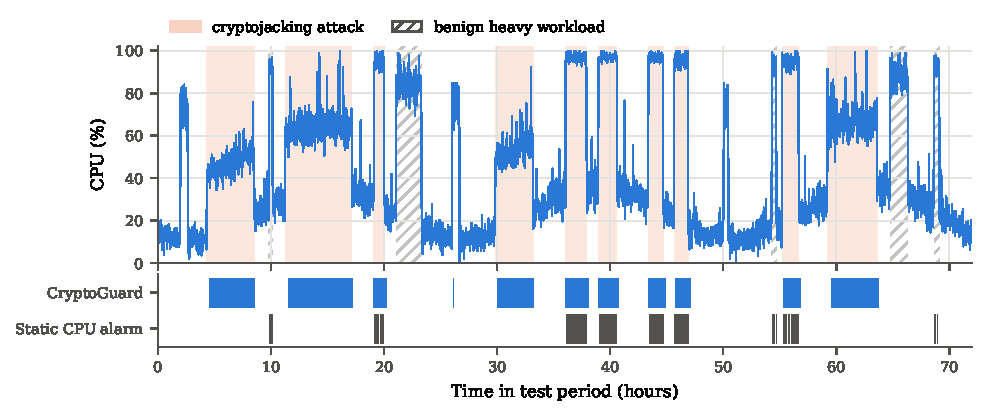
\includegraphics[width=\textwidth]{figures/timeline.pdf}
  \caption{One 3-day test run (seed 0). Top: CPU utilisation, attack periods and benign heavy workloads. Bottom: windows alerted by the static CPU alarm and by CryptoGuard. The static alarm misses every throttled miner and fires on a CI build; CryptoGuard alerts on every attack and on none of the benign workloads.}
  \label{fig:timeline}
\end{figure*}

\subsection{Ablation Study}
Table~\ref{tab:ablation} removes one component at a time. Without the CUSUM drift detector, most throttled miners are missed entirely. Without the XAI gate, every traffic surge and CI build becomes an alert, so false alerts per day rise sharply. Without threat-intelligence fusion, detection becomes slower because the behavioural evidence must be confirmed over several windows before it counts. Without the persistence filter, isolated spikes produce more false alerts. Without the maintenance window, the weekly report job inflates the CUSUM interval $h$, and the mean time to detect a throttled miner grows from \cgTTDstealthy{} to \nomwTTDstealthy{} minutes.

\begin{table}[t]
\caption{Ablation (mean over \nSeeds{} seeds). Det.\ thr.: throttled-miner detection rate; TTD in minutes for noisy / throttled / container miners}
\label{tab:ablation}
\centering
\scriptsize
\setlength{\tabcolsep}{2.6pt}
\resizebox{\columnwidth}{!}{%
\begin{tabular}{@{}lcccccccc@{}}
\toprule
Variant & F1 & \shortstack{Det.\\thr.} & \shortstack{Event\\det.} & \shortstack{TTD\\noisy} & \shortstack{TTD\\thr.} & \shortstack{TTD\\cont.} & FA/day & HN \\
\midrule
\textbf{CryptoGuard (full)} & 0.95 & 1.00 & 1.00 & 1.4 & 16 & 3.3 & 0.13 & 0.00 \\
\quad -- CUSUM drift detector & 0.49 & 0.12 & 0.66 & 1.4 & 176 & 3.3 & 0.07 & 0.00 \\
\quad -- XAI gate & 0.79 & 1.00 & 1.00 & 1.3 & 70 & 2.1 & 2.20 & 0.97 \\
\quad -- threat-intel fusion & 0.95 & 1.00 & 1.00 & 3.0 & 16 & 6.5 & 0.13 & 0.00 \\
\quad -- persistence filter & 0.95 & 1.00 & 1.00 & 1.0 & 15 & 2.5 & 1.13 & 0.00 \\
\quad -- maintenance window & 0.78 & 0.90 & 0.96 & 1.4 & 134 & 3.3 & 0.07 & 0.00 \\
\bottomrule

\end{tabular}}
\end{table}

\subsection{Sensitivity to the Gate Threshold}
Table~\ref{tab:gate} varies $\gamma$. A low gate ($\gamma=0.6$) lets part of the CI-build windows through. Between 0.7 and 0.8, the results are stable with almost no false alerts. A very strict gate starts to reject container-miner windows, whose attribution is partly on process churn, so the detection rate falls.

\begin{table}[t]
\caption{Effect of the XAI gate $\gamma$ (mean over \nSeeds{} seeds)}
\label{tab:gate}
\centering
\footnotesize
\begin{tabular}{@{}cccccc@{}}
\toprule
$\gamma$ & F1 & Event det. & TTD thr. (min) & FA/day & HN \\
\midrule
0.60 & 0.88 & 1.00 & 64 & 1.40 & 0.19 \\
0.70 & 0.94 & 1.00 & 29 & 0.20 & 0.00 \\
0.75 & 0.95 & 1.00 & 16 & 0.13 & 0.00 \\
0.80 & 0.96 & 1.00 & 8 & 0.27 & 0.00 \\
0.90 & 0.80 & 0.90 & 10 & 0.67 & 0.00 \\
\bottomrule

\end{tabular}
\end{table}

\subsection{Quality of Explanations}
Fig.~\ref{fig:xai} shows, for each scenario, how the SHAP attribution of anomalous windows is distributed over features. For all three miner families, the compute features carry at least \shareMinerMin{} of the attribution, and CPU excess is one of the two largest contributors. Traffic surges are explained mainly by connections, peers and throughput (compute share \shareSurge), which is exactly what the gate exploits. CI builds are explained partly by new processes and memory (compute share \shareCI). A typical alert for a throttled miner, produced \exStealthyMinute{} minutes into the attack, reads:

\begin{quote}\small\itshape
\exStealthySummary
\end{quote}

The alert names the three pieces of evidence an administrator would check and compares each with the server's own normal values, so the administrator does not have to trust a black-box score.

\begin{figure}[t]
  \centering
  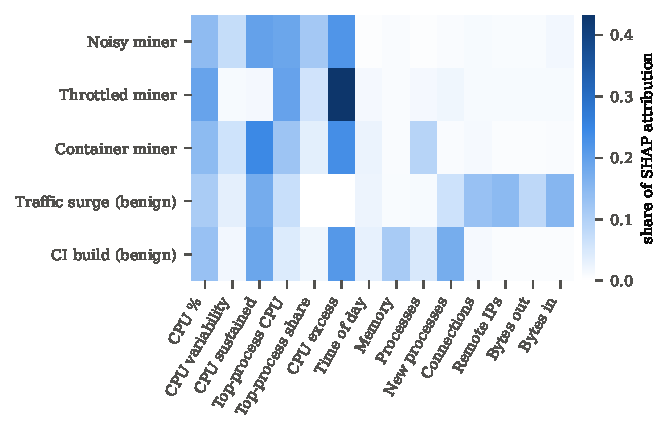
\includegraphics[width=\columnwidth]{figures/explanation_profile.pdf}
  \caption{Mean share of TreeSHAP attribution per feature for anomalous windows of each scenario (seed 0). Miners are explained by compute features; a traffic surge is explained by network features.}
  \label{fig:xai}
\end{figure}

\subsection{Automated Response}
Replaying the response policy on the test streams (Table~\ref{tab:response}), CryptoGuard contained \respContain\% of attacks by terminating the culprit or isolating the server, on average \respTTC{} minutes after the attack began. Across all seeds, it made \respWrongKill{} wrong kills and \respWrongIso{} wrong isolations per day. The kill-attribution rule matters: an earlier version that killed any non-allow-listed top process made occasional wrong kills in the minutes right after a miner stopped, when an ordinary worker briefly became the busiest process.

\begin{table}[t]
\caption{Automated response on the simulated streams (mean over \nSeeds{} seeds; TTC = time to containment)}
\label{tab:response}
\centering
\footnotesize
\setlength{\tabcolsep}{4pt}
\begin{tabular}{@{}lcccc@{}}
\toprule
Variant & Contained & TTC (min) & \shortstack{Wrong kills\\per day} & \shortstack{Wrong isol.\\per day} \\
\midrule
CryptoGuard (full) & 1.00 & 12.5$\pm$3.2 & 0.00 & 0.00 \\
No maint.\ window & 0.96 & 53.8$\pm$15.7 & 0.00 & 0.00 \\
\bottomrule

\end{tabular}
\end{table}

\subsection{Live Test}
CryptoGuard was also run end-to-end on a 2-vCPU Linux cloud container with active response (process termination on, network isolation off). A baseline of 120 windows of 5\,s was recorded (mean CPU 0.3\%), the model was trained on it, and the harmless miner simulator was then started twice. In the \emph{noisy} run (all cores, \texttt{xmrig} in the command line, connection to a fake pool on port 3333), the first alert came 0.8\,s after the miner started and the process was terminated after 0.8\,s. In the \emph{stealthy} run (one core at 50\%, no signature, no pool connection), detection relied on behaviour alone: the first alert came after 10.8\,s and the process was terminated after 91.5\,s, once the drift confidence passed the kill threshold. No alerts were raised in the windows before either miner started. Decisions are taken at the end of each window, so these latencies depend on when in a window the miner starts. The live test shows that the pipeline works end to end on a real host; it is not a measurement of accuracy, because the idle test host is far simpler than a production server.

The first alert of the stealthy run, raised from behaviour alone, read: \emph{Looks like cryptojacking because the server is using 25 percentage points more CPU than its current traffic and process activity can explain (normally under 1); CPU usage is 26\%, while this server normally runs at about 0\% at 15:00; a single process is using 25\% of total CPU (normal top process: ~0\%).}


% ==================================================================
\section{Discussion and Limitations}
% ==================================================================
\textbf{Synthetic data.} The main limitation is that the quantitative results come from a simulator. The simulator encodes assumptions---CPU proportional to load, miners that add a constant load, particular evasion rates---that favour detectors built on the same assumptions. The numbers should therefore be read as a controlled comparison of design choices, not as expected production accuracy. Validating CryptoGuard on real cloud telemetry with red-team miners is the most important next step.

\textbf{Adaptive attackers.} An attacker who knows the model could hide inside the learned noise, for example by mining only during traffic peaks with a few percent of the CPU, or by imitating a registered maintenance job. Such attacks would cut the attacker's profit sharply, which is itself a useful outcome, but they would not be detected. GPU mining and miners spread thinly across many containers are not covered by the current host-level features.

\textbf{Operational trade-offs.} The CUSUM interval is set by the heaviest legitimate compute job seen in training. Registering such jobs shortens detection time, but every registered window is also a place where drift evidence is not collected. Automatic process termination is safe only with good attribution, so CryptoGuard deliberately prefers ``alert only'' when it cannot attribute the excess CPU to a single process.

% ==================================================================
\section{Conclusion}
% ==================================================================
CryptoGuard shows that cryptojacking on cloud servers can be detected from ordinary host telemetry without attack labels, explained in terms an administrator can verify, and contained automatically with safeguards against harming legitimate workloads. Three design choices drive the results: a learned CPU-excess signal, two detection time-scales, and the use of SHAP explanations as a decision input rather than only as a display. Future work includes evaluation on real cloud telemetry, fleet-level baselines shared across similar instances, GPU and container-orchestrator signals, and integration with cloud-native response services.

\begin{thebibliography}{99}
\bibitem{google2021threat}
Google Cybersecurity Action Team, ``Threat Horizons: Cloud Threat Intelligence,'' Google Cloud, Rep.~1, Nov.~2021.

\bibitem{sysdig2022}
Sysdig Threat Research Team, ``2022 Sysdig Cloud-Native Threat Report,'' Sysdig, Inc., Sep.~2022.

\bibitem{mitre_t1496}
The MITRE Corporation, ``Resource Hijacking, Technique T1496,'' MITRE ATT\&CK. [Online]. Available: https://attack.mitre.org/techniques/T1496/

\bibitem{tekiner2021sok}
E.~Tekiner, A.~Acar, A.~S.~Uluagac, E.~Kirda, and A.~A.~Selcuk, ``SoK: Cryptojacking malware,'' in \emph{Proc. IEEE European Symp. Security and Privacy (EuroS\&P)}, 2021, pp.~120--139.

\bibitem{pastor2020}
A.~Pastor, A.~Mozo, S.~Vakaruk, D.~Canavese, D.~R.~L\'opez, L.~Regano, S.~G\'omez-Canaval, and A.~Lioy, ``Detection of encrypted cryptomining malware connections with machine and deep learning,'' \emph{IEEE Access}, vol.~8, pp.~158036--158055, 2020.

\bibitem{eskandari2018}
S.~Eskandari, A.~Leoutsarakos, T.~Mursch, and J.~Clark, ``A first look at browser-based cryptojacking,'' in \emph{Proc. IEEE European Symp. Security and Privacy Workshops (EuroS\&PW)}, 2018, pp.~58--66.

\bibitem{konoth2018minesweeper}
R.~K.~Konoth, E.~Vineti, V.~Moonsamy, M.~Lindorfer, C.~Kruegel, H.~Bos, and G.~Vigna, ``MineSweeper: An in-depth look into drive-by cryptocurrency mining and its defense,'' in \emph{Proc. ACM SIGSAC Conf. Computer and Communications Security (CCS)}, 2018, pp.~1714--1730.

\bibitem{chandola2009}
V.~Chandola, A.~Banerjee, and V.~Kumar, ``Anomaly detection: A survey,'' \emph{ACM Computing Surveys}, vol.~41, no.~3, pp.~1--58, 2009.

\bibitem{liu2008iforest}
F.~T.~Liu, K.~M.~Ting, and Z.-H.~Zhou, ``Isolation forest,'' in \emph{Proc. 8th IEEE Int. Conf. Data Mining (ICDM)}, 2008, pp.~413--422.

\bibitem{scholkopf2001}
B.~Sch\"olkopf, J.~C.~Platt, J.~Shawe-Taylor, A.~J.~Smola, and R.~C.~Williamson, ``Estimating the support of a high-dimensional distribution,'' \emph{Neural Computation}, vol.~13, no.~7, pp.~1443--1471, 2001.

\bibitem{page1954}
E.~S.~Page, ``Continuous inspection schemes,'' \emph{Biometrika}, vol.~41, no.~1/2, pp.~100--115, 1954.

\bibitem{ribeiro2016}
M.~T.~Ribeiro, S.~Singh, and C.~Guestrin, ```Why should I trust you?': Explaining the predictions of any classifier,'' in \emph{Proc. 22nd ACM SIGKDD Int. Conf. Knowledge Discovery and Data Mining}, 2016, pp.~1135--1144.

\bibitem{lundberg2017}
S.~M.~Lundberg and S.-I.~Lee, ``A unified approach to interpreting model predictions,'' in \emph{Advances in Neural Information Processing Systems 30 (NeurIPS)}, 2017, pp.~4765--4774.

\bibitem{lundberg2020trees}
S.~M.~Lundberg, G.~Erion, H.~Chen, A.~DeGrave, J.~M.~Prutkin, B.~Nair, R.~Katz, J.~Himmelfarb, N.~Bansal, and S.-I.~Lee, ``From local explanations to global understanding with explainable AI for trees,'' \emph{Nature Machine Intelligence}, vol.~2, no.~1, pp.~56--67, 2020.

\bibitem{pedregosa2011}
F.~Pedregosa \emph{et al.}, ``Scikit-learn: Machine learning in Python,'' \emph{Journal of Machine Learning Research}, vol.~12, pp.~2825--2830, 2011.
\end{thebibliography}

\end{document}
